\section{Cuboidal Die}
Our first approach at making a die was the cuboidal die. The reasoning behind this is that the number of parameters for a cuboidal die is significantly lower. A cuboidal die has only three parameters, the length, breadth and height. If we make the assumption that the discrepancy of a die does not change significantly with scale (as we do in this section), then simply make one of the three parameters constant so that we only have two parameters. We got past this assumption by building multiple dice with the final parameters with different scales so that we could pick the one with the best discrepancy.\\
\subsubsection{Theoretical Analysis}
The first important observation about cuboidal dice is that the opposite faces have equal probabilities. So now we have the probabilities of the six faces to be $p_a, p_a, p_b, p_b, p_c, p_c$. In our analysis for all six faced dice, we had six different probabilities that we treated as a binary string with each digit in the string representing whether the corresponding face was included in the subset or not. We then considered the total number of subsets to arrive at the best theoretical discrepancy. In this case, we do something similar.\\
Since each probability is either present once, twice or not present, we represent each subset of probabilities as a base-3 string having three digits for the three distinct probabilities. We then get the different subsets as:\\
000 = 0\\
001 = $p_a$\\
002 = $2p_a$\\
010 = $p_b$\\
$\ldots$\\
201 = $2p_c + p_a$\\
$\ldots$\\
222 = $2p_c + 2p_b + 2p_a$\\
The optimal discrepancy for this die is when: a. All these values are distinct and b. The difference between each consecutive value is the same.\\
Since there are $3^3 = 27$ total number of subsets, we divide the region 0 to 1 into 27 points including zero and one. So the subsets are now: $0, \frac{1}{26},\ \frac{2}{26}, \ldots \frac{25}{26},\ 1$. Clearly one of the three probabilities must be $\frac{1}{26}$ because it is the smallest probability. Going from there, the next probability that we cannot reach is $\frac{3}{26}$ so we set one of our probabilities to that value. The optimal optimal values for $p_a, p_b$ and $p_c$ that satisfy this constraint are $p_a = \frac{1}{26},\ p_b = \frac{3}{26}$ and $p_c = \frac{9}{26}$. With these values all the subsets are different and the difference between two consecutive subsets is the same, which makes these the optimal values for the constraint that every opposite side has the same probability.\\

\subsubsection{Algorithm to Reach Optimal Dice}
The hardest part of the dice project is finding exactly how the dice values change with changes in length, angle or weights.\\
In the case of cuboidal dice, it was actually possible to develop a deterministic algorithm to reach the optimal dice parameters.\\
Consider that $q_a, q_b$ and $q_c$ are the measured probabilities of the dice such that $q_a < q_b < q_c$.\\
The target values for $(q_a, q_b, q_c)$ are $(\frac{1}{26}, \frac{3}{26}, \frac{9}{26})$.\\
Let us examine what happens to the probabilities if we change one of the three parameters.\\
Consider that $h < b < l$. Clearly, $(q_a, q_b, q_c)$ correspond to the faces (bh, lh, lb) because the face area.\\
If we increase l, the faces lh and lb increase. So the probabilities $q_b$ and $q_c$ increase by some amount and $q_a$ decreases. We don't really care about the amount that they change by, the mere fact that we know which faces increase and which decrease is enough to develop the strategy.\\
Similarly, if we increase edge b, the probabilities for faces lb and bh will increase and lh will decrease. It is the same for edge h.\\
A similar argument can be made for decreasing the edge length as well, the opposite will happen.\\
Note that this approach assumes that given a die, the exact value probability values for the faces can be calculated.\\
Now we describe the strategy to reach the optimal value:\\
\begin{itemize}
    \item Pick l = b = h\\
    \item Measure the probabilities of the faces bh, lh, lb. Their target values are $(\frac{1}{26}, \frac{3}{26}, \frac{9}{26})$.\\
    \item Suppose lb and lh are both greater than their target. This means bh is less than its target. Decrease the side l by as much as possible to bring them closer to the optimal value. This will bring all three faces closer to the optimal value.\\
    Similarly, if lb and lh are both less than their target, increase l.\\
    \item Note that this works irrespective of which two faces are greater or less than their target.\\

\end{itemize}

Note that this algorithm will converge when one of the three faces reaches their target, not when all three reach. We can fix this by using two binary searches, one on the lb face's probability and one on lh face's probability (when both of these reach their target, bh will also reach the target). However, we did not implement the two binary searches because finding the probabilities of each face with a high enough accuracy to justify using this was anyway not possible, especially on a simulator.\\

\subsubsection{Simulator Values}
We ran the simulator for 10000 rolls at every possible initial orientation to generate an estimate of the probabilities. We decided to limit our search to only integer length edges and reached an optimal value of length, breadth and height of values 12, 11 and 9. The probabilities for these faces were as follows:\\
Six sided cuboid die simulation result:\\
calculated probs for side 1: 0.05 (9.4\%)\\
calculated probs for side 2: 0.338 (25.6\%)\\
calculated probs for side 3: 0.107 (16.4\%)\\
calculated probs for side 4: 0.359 (28.6\%)\\
calculated probs for side 5: 0.105 (11.6\%)\\
calculated probs for side 6: 0.041(8.4\%)\\
calculated discrepancy: 0.0205\\
The calculated discrepancy for the simulation of this dice was 0.0205. This was close enough to the optimal value of $\frac{1}{52}$ = 0.0192 that we did not experiment with non integer values.\\

\subsubsection{Pre-Tournament Rolling Analysis}
After reducing the problem to one in which the surface areas of parallel surfaces were the same and calculating an optimal build with proportions of 9x11x12, we proceeded to 3d-print three dice with the previously mentioned dimensions for testing in sizes scaled 1x, 2x and 3x. We 3d-printed the same die in three different sizes because of uncertainties regarding how scale would affect our calculated probabilities in the real world.\\
‘Small’ dice corresponds to 1x the proportions. ‘Medium’ dice corresponds to 2x the proportions. And lastly, ‘Large’ dice corresponds to 3x the proportions. Each die was rolled 100 times into a cardboard box. The top side of the die was recorded after each throw. For each die: 6 pips and 1 pip correspond to sides that are proportionally 11x12, 5 pips and 2 pips correspond to sides that are proportionally 12x9, 3 pips and 4 pips correspond to sides that are proportionally 9x11. Our real-world results for these three die were as follows.\\

Total Rolls for 'Small' ( cuboid ): 100\\
Measured frequency for side 1: 22\\
Measured frequency for side 2: 12\\
Measured frequency for side 3: 8\\
Measured frequency for side 4: 10\\
Measured frequency for side 5: 15\\
Measured frequency for side 6: 33\\
Discrepancy: 4\%\\

Total Rolls for 'Medium' ( cuboid ): 100\\
Measured frequency for side 1: 34\\
Measured frequency for side 2: 15\\
Measured frequency for side 3: 7\\
Measured frequency for side 4: 8\\
Measured frequency for side 5: 13\\
Measured frequency for side 6: 23\\
Discrepancy: 3.5\%\\

Total Rolls for 'Large' ( cuboid ): 100\\
Measured frequency for side 1: 31\\
Measured frequency for side 2: 12\\
Measured frequency for side 3: 11\\
Measured frequency for side 4: 11\\
Measured frequency for side 5: 16\\
Measured frequency for side 6: 19\\
Discrepancy: 5.5\%\\

The results showed consistency across our scaled die with our simulated results. For any of the die, when the faces are sorted in increasing order according to their associated recorded probabilities, each face sits adjacent to its parallel face.//
Because the 'Medium' sized die demonstrated the closest adherence to our simulated results, we chose it for the tournament.

\subsubsection{Post-Tournament Rolling Analysis}
\begin{figure}[h]
\center
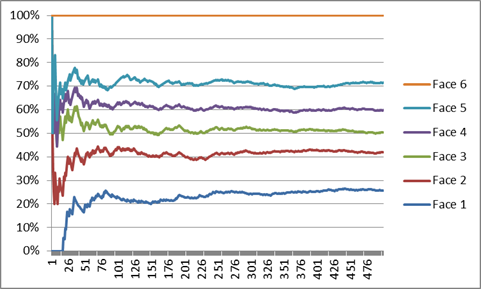
\includegraphics[scale=1]{cuboid_graph.png}
\caption{Probability shares for each face as a function of rolls. The gap between lines is the probablity of each face.}
\label{fig:cuboid}
\end{figure}
\begin{figure}[h]
\center
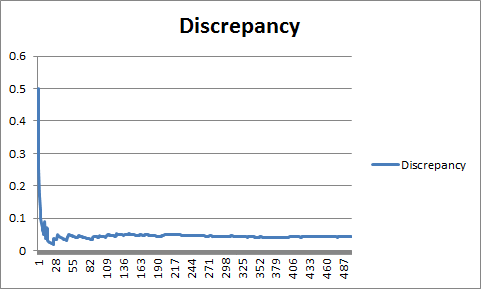
\includegraphics[scale=1]{cuboid_di.png}
\caption{Measured discrepancy as a function of number of rolls.}
\label{fig:cuboid}
\end{figure}
Total Rolls ( cuboid ): 500\\
Measured frequency for side 1: 128\\
Measured frequency for side 2: 82\\
Measured frequency for side 3: 42\\
Measured frequency for side 4: 47\\
Measured frequency for side 5: 58\\
Measured frequency for side 6: 143\\
Discrepancy: 4.2\%\\
The measured discrepancy turned out to be 4.2\%, which is about twice what was calculated by the simulator. There are two main reasons we believe led to this difference:\\
\begin{itemize}
    \item Inaccuracies inherent in the simulator that arise from a lack of data about friction and the restitution of the rolling surface. There are also inaccuracies that arise from the simulator cutting corners to improve speed.\\
    \item Our usage of a 20\% fill for the 3D printed dice. As we discuss later, a 100\% fill for the five sided dice led to a very accurate result.
\end{itemize}
